\documentclass{ximera}


\graphicspath{
  {./}
  {ximeraTutorial/}
  {basicPhilosophy/}
}

\newcommand{\mooculus}{\textsf{\textbf{MOOC}\textnormal{\textsf{ULUS}}}}

\usepackage{tkz-euclide}\usepackage{tikz}
\usepackage{tikz-cd}
\usetikzlibrary{arrows}
\tikzset{>=stealth,commutative diagrams/.cd,
  arrow style=tikz,diagrams={>=stealth}} %% cool arrow head
\tikzset{shorten <>/.style={ shorten >=#1, shorten <=#1 } } %% allows shorter vectors

\usetikzlibrary{backgrounds} %% for boxes around graphs
\usetikzlibrary{shapes,positioning}  %% Clouds and stars
\usetikzlibrary{matrix} %% for matrix
\usepgfplotslibrary{polar} %% for polar plots
\usepgfplotslibrary{fillbetween} %% to shade area between curves in TikZ
\usetkzobj{all}
\usepackage[makeroom]{cancel} %% for strike outs
%\usepackage{mathtools} %% for pretty underbrace % Breaks Ximera
%\usepackage{multicol}
\usepackage{pgffor} %% required for integral for loops



%% http://tex.stackexchange.com/questions/66490/drawing-a-tikz-arc-specifying-the-center
%% Draws beach ball
\tikzset{pics/carc/.style args={#1:#2:#3}{code={\draw[pic actions] (#1:#3) arc(#1:#2:#3);}}}



\usepackage{array}
\setlength{\extrarowheight}{+.1cm}
\newdimen\digitwidth
\settowidth\digitwidth{9}
\def\divrule#1#2{
\noalign{\moveright#1\digitwidth
\vbox{\hrule width#2\digitwidth}}}






\DeclareMathOperator{\arccot}{arccot}
\DeclareMathOperator{\arcsec}{arcsec}
\DeclareMathOperator{\arccsc}{arccsc}

















%%This is to help with formatting on future title pages.
\newenvironment{sectionOutcomes}{}{}


\title{Volume}

\begin{document}

\begin{abstract}
cubic units
\end{abstract}
\maketitle



We can also measure volume and how it changes.



\[
\text{rate} = \frac{\Delta \text{volume}}{\Delta \text{time}} 
\]








\subsection{Conical Tank}

A conical tank (with vertex down) is 12 feet across and 14 fee deep. If water is flowing into the tank at a rate of 9 cubic feet per minute, find the rate of change of the depth of the water when the water is 8 feet deep.






\textbf{\textcolor{purple!85!blue}{Step 1: A Picture}}


\begin{image}
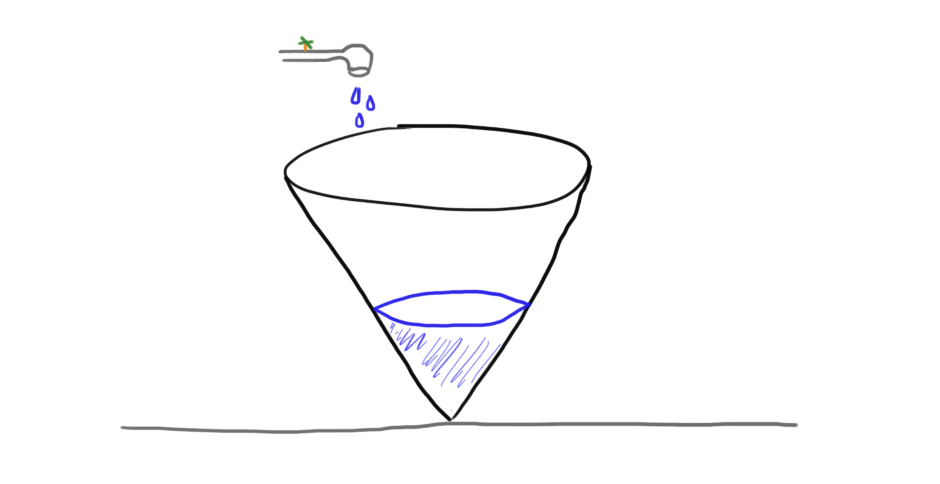
\includegraphics{pics/cone_1.png}
\end{image}




\textbf{\textcolor{purple!85!blue}{Step 2: Identify Measurements}}






\begin{image}
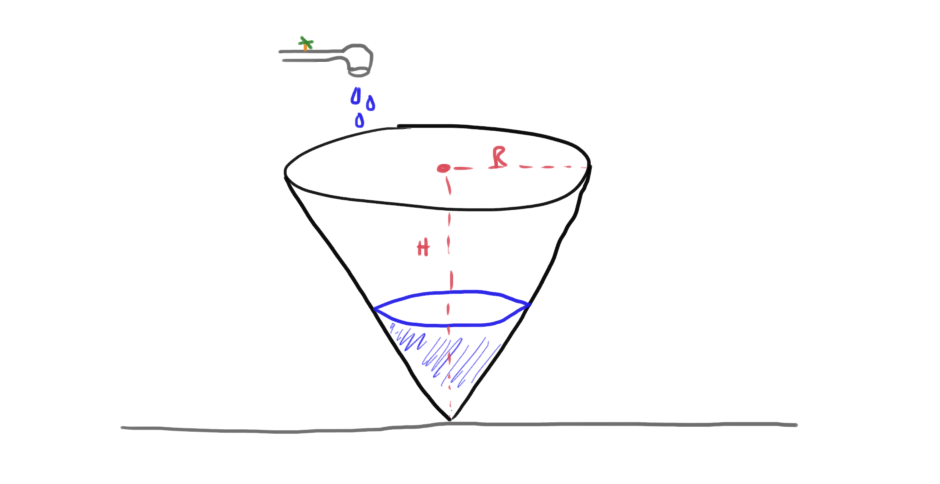
\includegraphics{pics/cone_3.png}
\end{image}






$\blacktriangleright$ We begin with two pertinent lengths that remain constant throughout the story:

\begin{itemize}
\item $R$ is the radius of the base of the conical tank.
\item $H$ is the height of the conical tank.
\end{itemize}

These are constant functions of time, $t$: $R(t)$ and $H(t)$.







\begin{question} $\boxdot$ 

As water pours into the tank, what shape does the water take?

\begin{multipleChoice}
\choice {Triangle}
\choice {Sphere}
\choice[correct] {Cone}
\choice {Rectangular Prism}
\end{multipleChoice}

\end{question}









\begin{question} $\boxdot$ 

As water pours into the tank, how does the height of the water change?

\begin{multipleChoice}
\choice[correct] {Increases}
\choice {Decreases}
\choice {Remains Constant}
\end{multipleChoice}

\end{question}







\begin{question} $\boxdot$ 

As water pours into the tank, how does the radius of the water base change?

\begin{multipleChoice}
\choice[correct] {Increases}
\choice {Decreases}
\choice {Remains Constant}
\end{multipleChoice}

\end{question}









\textbf{\textcolor{purple!85!blue}{Step 3: Water Measurements}}


As water pours into the tank the water level rises.  The water also forms a cone and the height and radius both increase.  








\begin{image}
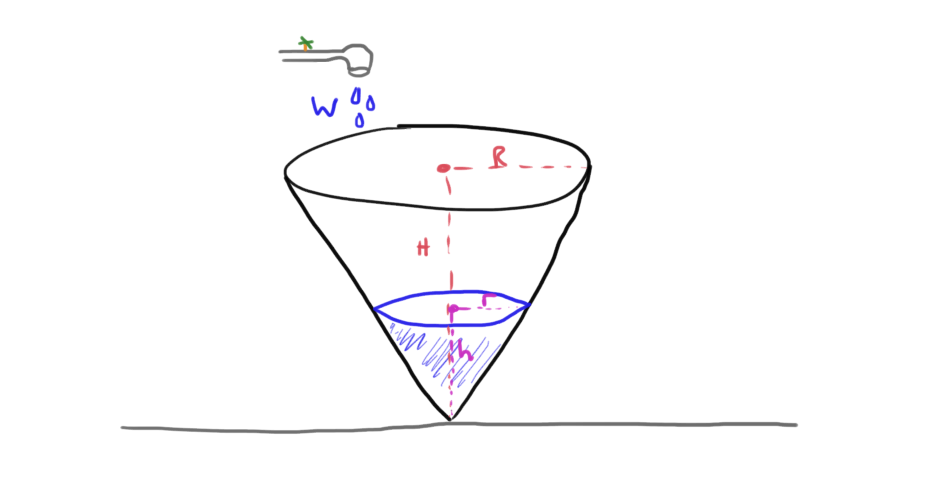
\includegraphics{pics/cone_4.png}
\end{image}





$\blacktriangleright$ We need to represent these measurements as well:

\begin{itemize}
\item $r$ is the radius of the base of the conical water.
\item $h$ is the height of the conical water.
\end{itemize}

These are increasing functions of time, $t$: $r(t)$ and $h(t)$.










\textbf{\textcolor{purple!85!blue}{Step 3: Geometric Relationships}}


Our measurements are vertical and horizontal measurements.  If we take these with the side of the tank, they make a right triangle.  In fact, they make two similar right triangles.






\begin{image}
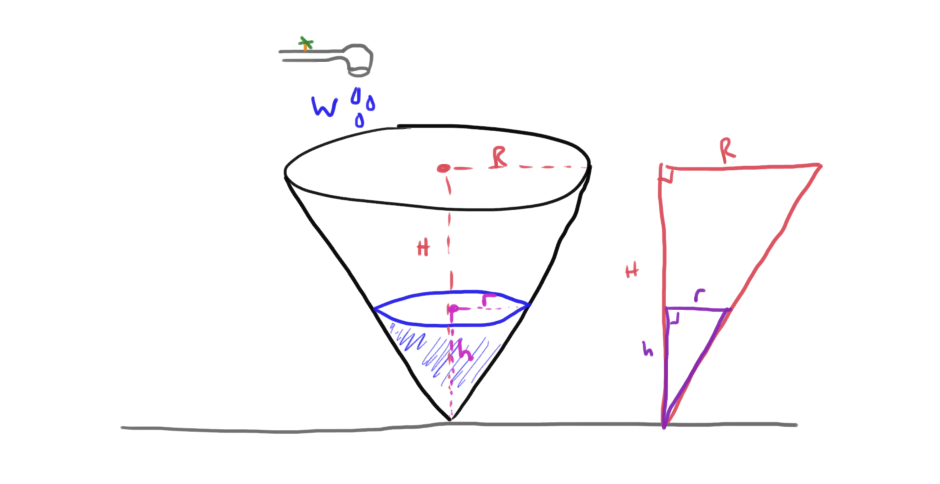
\includegraphics{pics/cone_5.png}
\end{image}




$\blacktriangleright$ Similar Triangles



\[
\frac{H}{R} = \frac{h}{r}
\]


From this relationship, we can get expressions for $h$ or $r$ in terms of the others. 



\[
h = \frac{r \, H}{R} \, \text{ and } \,  r = \frac{h \, R}{H}
\]







$\blacktriangleright$ Volume


We are also given information about the volume.  Therefore, we should be thinking about the volume of cones.

\[
V = \frac{1}{3} \pi \, r^2 \, h
\]







We are just modeling here, which means collecting as many descriptions and relationships as we can. \\

We'll leave answering the question for later.






\end{document}
